\def\year{2020}\relax
%File: formatting-instruction.tex
\documentclass[letterpaper]{article} % DO NOT CHANGE THIS
\usepackage{aaai20}  % DO NOT CHANGE THIS
\usepackage{times}  % DO NOT CHANGE THIS
\usepackage{helvet} % DO NOT CHANGE THIS
\usepackage{courier}  % DO NOT CHANGE THIS
\usepackage[hyphens]{url}  % DO NOT CHANGE THIS
\usepackage{graphicx} % DO NOT CHANGE THIS
\urlstyle{rm} % DO NOT CHANGE THIS
\def\UrlFont{\rm}  % DO NOT CHANGE THIS
\usepackage{graphicx}  % DO NOT CHANGE THIS
\frenchspacing  % DO NOT CHANGE THIS
\setlength{\pdfpagewidth}{8.5in}  % DO NOT CHANGE THIS
\setlength{\pdfpageheight}{11in}  % DO NOT CHANGE THIS
%\usepackage[UTF8]{ctex}
\usepackage{booktabs} %table topline,midline,bottomline
\usepackage{algorithm}
\usepackage{algorithmicx}
%\nocopyright
%PDF Info Is REQUIRED.
% For /Author, add all authors within the parentheses, separated by commas. No accents or commands.
% For /Title, add Title in Mixed Case. No accents or commands. Retain the parentheses.
 \pdfinfo{
/Title (Synthesis of Registered Brain Multimodal MRI with Lesions)
/Author (Yili Qu,Wanqi Su,Chufu Deng,Ying Wang,Yutong Lu,Zhiguang Chen,Nong Xiao)
} %Leave this	
% /Title ()
% Put your actual complete title (no codes, scripts, shortcuts, or LaTeX commands) within the parentheses in mixed case
% Leave the space between \Title and the beginning parenthesis alone
% /Author ()
% Put your actual complete list of authors (no codes, scripts, shortcuts, or LaTeX commands) within the parentheses in mixed case. 
% Each author should be only by a comma. If the name contains accents, remove them. If there are any LaTeX commands, 
% remove them. 

% DISALLOWED PACKAGES
% \usepackage{authblk} -- This package is specifically forbidden
% \usepackage{balance} -- This package is specifically forbidden
% \usepackage{caption} -- This package is specifically forbidden
% \usepackage{color (if used in text)
% \usepackage{CJK} -- This package is specifically forbidden
% \usepackage{float} -- This package is specifically forbidden
% \usepackage{flushend} -- This package is specifically forbidden
% \usepackage{fontenc} -- This package is specifically forbidden
% \usepackage{fullpage} -- This package is specifically forbidden
% \usepackage{geometry} -- This package is specifically forbidden
% \usepackage{grffile} -- This package is specifically forbidden
% \usepackage{hyperref} -- This package is specifically forbidden
% \usepackage{navigator} -- This package is specifically forbidden
% (or any other package that embeds links such as navigator or hyperref)
% \indentfirst} -- This package is specifically forbidden
% \layout} -- This package is specifically forbidden
% \multicol} -- This package is specifically forbidden
% \nameref} -- This package is specifically forbidden
% \natbib} -- This package is specifically forbidden -- use the following workaround:
% \usepackage{savetrees} -- This package is specifically forbidden
% \usepackage{setspace} -- This package is specifically forbidden
% \usepackage{stfloats} -- This package is specifically forbidden
% \usepackage{tabu} -- This package is specifically forbidden
% \usepackage{titlesec} -- This package is specifically forbidden
% \usepackage{tocbibind} -- This package is specifically forbidden
% \usepackage{ulem} -- This package is specifically forbidden
% \usepackage{wrapfig} -- This package is specifically forbidden
% DISALLOWED COMMANDS
% \nocopyright -- Your paper will not be published if you use this command
% \addtolength -- This command may not be used
% \balance -- This command may not be used
% \baselinestretch -- Your paper will not be published if you use this command
% \clearpage -- No page breaks of any kind may be used for the final version of your paper
% \columnsep -- This command may not be used
% \newpage -- No page breaks of any kind may be used for the final version of your paper
% \pagebreak -- No page breaks of any kind may be used for the final version of your paperr
% \pagestyle -- This command may not be used
% \tiny -- This is not an acceptable font size.
% \vspace{- -- No negative value may be used in proximity of a caption, figure, table, section, subsection, subsubsection, or reference
% \vskip{- -- No negative value may be used to alter spacing above or below a caption, figure, table, section, subsection, subsubsection, or reference

\setcounter{secnumdepth}{2} %May be changed to 1 or 2 if section numbers are desired.

% The file aaai20.sty is the style file for AAAI Press 
% proceedings, working notes, and technical reports.
%
\setlength\titlebox{2.5in} % If your paper contains an overfull \vbox too high warning at the beginning of the document, use this
% command to correct it. You may not alter the value below 2.5 in
\title{Synthesis of Registered Multimodal Brain MRI with Lesions}
%Your title must be in mixed case, not sentence case. 
% That means all verbs (including short verbs like be, is, using,and go), 
% nouns, adverbs, adjectives should be capitalized, including both words in hyphenated terms, while
% articles, conjunctions, and prepositions are lower case unless they
% directly follow a colon or long dash
%%%\author{\Large \textbf{Yili Qu,Wanqi Su,Chufu Deng,}\\ \Large \textbf{Ying Wang,Yutong Lu,Nong Xiao,Zhiguang Chen}\\  % All authors must be in the same font size and format. Use \Large and \textbf to achieve this result when breaking a line
 %If you have multiple authors and multiple affiliations
% use superscripts in text and roman font to identify them. For example, Sunil Issar,\textsuperscript{\rm 2} J. Scott Penberthy\textsuperscript{\rm 3} George Ferguson,\textsuperscript{\rm 4} Hans Guesgen\textsuperscript{\rm 5}. Note that the comma should be placed BEFORE the superscript for optimum readability
%%%School of Data and Computer Science\\ Sun Yet-Sen University\\	
%%%quyli@mail2.sysu.edu.cn% email address must be in roman text type, not monospace or sans serif
%%%}
\begin{document}

\maketitle

\begin{abstract}
In a large number of data-driven medical image intelligent processing tasks, the collection and acquisition of medical image data is very difficult, especially the registered multimodal medical image data. Synthetic medical image data can well alleviate the problem of insufficient data. In this paper, based on the unsupervised conditional GAN model, we achieve the generation of registered multimodal medical images from random normal distribution matrix and corresponding lesion information can be efficiently generated based on the freely selected lesion label. We conduct a number of validation experiments on BRATS2015 to verify that our synthetic MRI can be used as pre-trained data or enhanced data in medical image intelligent processing tasks, and can greatly improve generalization ability of the model.
\end{abstract}
	
\section{Introduction}
MRI is a common medical image that can have multiple modalities depending on imaging parameters, such as T1, T2, T1c and so on. Different modalities have different reference values for doctors. To make accurate judgments, doctors often need multiple modal images to compare with each other. In training and learning of medical image intelligent processing tasks, we often expect to obtain more modal images, such as medical image processing tasks based on CNN\cite{86krizhevsky2012imagenet} or GAN\cite{25goodfellow2014generative}. 

When obtaining different modalities from the same part of the same patient through different imaging techniques, these modalities are considered to be registered if the imaging position and the viewing angle are identical. Compared with unimodal data, the registered multimodal image data can provide more information, support more complex application scenarios, meet the training data requirements of deep neural networks, and help to provide intelligent diagnostic services more efficient and more reliable. For doctors, it takes longer to acquire images of different modalities and requires patient patience. For researchers of medical image intelligent processing tasks, multimodal MRI datasets are scarce, and the collection is very difficult, especially rare disease data, and the registered data is even rarer, which makes many training tasks impossible. Therefore, the application of image synthesis technology to extend datasets, translate existing unimodal images to registered multimodal images, or generate registered multimodal images from random noise matrix, has a wide range of uses and far-reaching significance.

Before the popularity of GAN, researchers focused on existed medical image modality translate to other modalities\cite{22burgos2015robust,33huang2017simultaneous,34vemulapalli2015unsupervised,36vannguyen2015crossdomain}. After GAN has shown its powerful generation ability, there are many researches on medical image translation based on GAN\cite{2zhang2018translating,20nie2017medical,35osokin2017gans,36vannguyen2015crossdomain,40kamnitsas2017unsupervised}. Many studies use GAN to achieve higher translation quality\cite{1zhao2018modular,5liang2018generative,6zhu2017unpaired,13choi2018stargan:}. Recent studies have implemented the translation on unregistered multimodal data\cite{2zhang2018translating,85joyce2017robust}.
GAN has been gradually applied to various organs, such as brain MRI to CT translation\cite{20nie2017medical,40kamnitsas2017unsupervised}, retinal vascular annotation to image translation\cite{41costa2017towards}, cardiac MRI to CT translation and segmentation using unsupervised CycleGAN\cite{6zhu2017unpaired,20nie2017medical}.
For multimodal image synthesis, \cite{84chartsias2018multimodal} implements multi-input and multi-output MRI synthesis, but registration is required for input multimodal data. \cite{85joyce2017robust} further implements an unregistered multi-input synthesis model, which can perform image synthesis from any subset of its input, but limits the output to unimodal. \cite{66Miao2018dilated} studies for medical image registration in-depth. \cite{4shin2018medical} uses GAN to synthesize brain tumor images to enhance data and anonymize data, but requires additional training of anatomical structure segmentation network.
Besides,\cite{41costa2017towards} implements the random generation of vascular annotation maps based on the idea of variational auto-encoder (VAE)\cite{87kingma2014auto-encoding}, and then synthesizes color retinal images based on the vascular annotation maps.
Beyond the field of medical image processing, the research of multi-domain translation is very active\cite{1zhao2018modular,5liang2018generative,13choi2018stargan:,27isola2017image-to-image}.
But in the field of medical image synthesis, there still are many researches of translation synthesis on two-modal\cite{2zhang2018translating,20nie2017medical,22burgos2015robust,34vemulapalli2015unsupervised,35osokin2017gans,36vannguyen2015crossdomain,40kamnitsas2017unsupervised}, and rare research on multimodal\cite{84chartsias2018multimodal,85joyce2017robust,4shin2018medical}.

At present, there are various problems in the research of medical image synthesis, such as the difficulty of expanding the number of modalities, the need to registered training data, relying on complex large networks, the inability to add or retain lesions, the inability to generate from random matrix, and the need of additional training data, etc. Moreover, the evaluation of synthetic data in most studies relies on the artificial visual effects assessment by experienced physicians, without objective quantitative evaluation. Therefore, we design a registered multimodal MRI generation scheme based on the Conditional Generative Adversarial Networks (CGAN)\cite{70mirza2014conditional}. With unsupervised learning method, training data does not need to be registered. Our solution can receive a random normal distribution matrix as input to generate a set of registered multimodal MRI with setted lesions. We perform multimodal brain MRI generation experiments with tumor segmentation labels on BRATS2015, and verify the effectiveness of lesion information and the availability of synthetic data in tumor lesion segmentation experiments. We will open the code. In general, our contribution is in the following three aspects:

\begin{itemize}
	\item \textbf{Extraction \& Generation of Structural Feature Map}
	We propose an extraction method for anatomical structure features of medical images. Without additional anatomical segmentation labels or label extraction training, structural feature maps can be extracted directly from real images of arbitrary modalities. The extraction method can improve the quality of synthetic images without introducing additional parameters and computation overhead. We also train a structural feature map generator to generate structural feature maps from multidimensional normal distribution. The random generation method can generate rich and diverse structural feature maps indefinitely.
	\item \textbf{Synthesis of Registered Multimodal MRI with Lesions}
	We use randomly generated structural feature maps to fuse with random lesion labels and then synthesize the registered multimodal MRI through the generator. We explore a variety of lesion generation guidance methods to achieve effective mapping of lesions based on input lesion labels during multimodal MRI synthesis. In training, no registered data is required except for the lesion labels. The synthetic data is registered, and the input lesion label is the lesion label of the synthetic data. Our solution enables fast and easy construction of registered multimodal MRI datasets with lesions label.
	\item \textbf{Objective Verification for Synthetic Data Availability}
	We construct datasets with different amounts of synthetic and real data to train the lesion segmentor, and verify that the synthetic data can be used as pre-training data and enhanced data in medical image intelligent processing tasks to improve generalization ability of the model and improve segmentation precision. Compared with traditional subjective evaluation method of synthetic image quality, we present the availability of synthetic data in intelligent lesion processing tasks more objectively.
\end{itemize}


\section{Method}
\label{method}
We perform our scheme on multimodal brain MRI synthesis task , in which the synthetic lesions are tumors, the lesion processing task is lesion segmentation, and the lesion label is a tumor segmentation label. Our scheme does not limit the body parts, lesion types, lesion processing tasks, specific modality and the number of modalities. We can easily apply this method to other similar tasks.
\subsection{Architecture}
\begin{figure}[t]
	\centering
	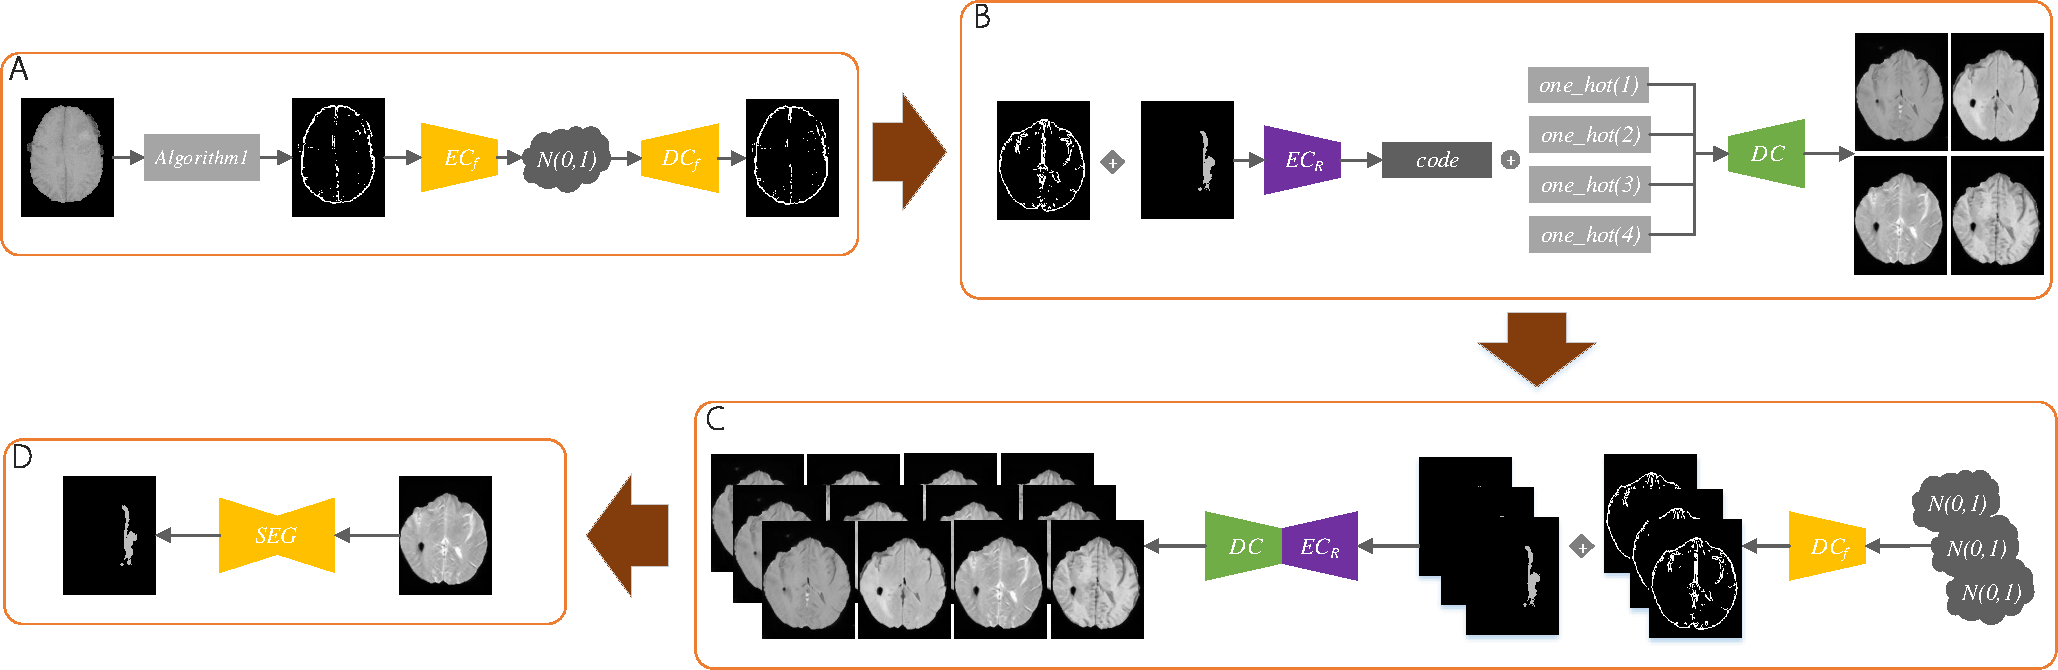
\includegraphics[width=0.95\columnwidth]{figures/architecture}
	\caption{Architecture.}
	\label{architecture}
\end{figure}
As shown in Fig.~\ref{architecture}, our scheme includes four main stages. 
In the structural feature map extraction and generation stage, we will obtain a structural feature map generator that can generate structural feature maps from random normal distribution matrix. 
In the multimodal MRI generation stage, we train a conditional generator with input of structural feature maps and lesion labels, which can generate MRI of different modalities according to different one-hot conditional matrixes.
In the synthetic datasets construction stage, we use the models produced in the first two stages to generate registered multimodal MRI from random normal distribution matrixes. 
In the synthetic data availability verification stage, we train and test the lesion segmentors on different datasets constructed from different amounts of synthetic data and real data.

\subsection{Structural Feature Map Extraction Method}
Medical images generated directly from random noise by GAN are often difficult to train and difficult to generate real structural information. We call image that provids basic contour and structure information as structural feature map. For example, a retinal vascular distribution map can be regarded as a structural feature map of a retinal image\cite{41costa2017towards}. Structural feature maps can provide necessary basic guidance for the synthesis of medical images. When synthesizing brain MRI, some studies obtains basic structural information from the brain segmentation labels\cite{4shin2018medical}. However, general structural features such as retinal vascular maps and brain segmentation labels require additional data and training before extracting from the original image. To this end, we first design a method for extracting structural feature maps directly from brain MRI, which has the advantages of fast operation, no training, no additional data.

In the traditional digital image processing methods, Roberts operator, Prewitt operator, Sobel operator, etc. are excellent edge detection operators. Sobel operator is often used in processing of brain medical images. As shown in Algorithm~\ref{alg:1}, we explore a method to further extract structural feature maps from the edge detection maps generated by Sobel operator.
\begin{algorithm}
	\caption{Structural Feature Extraction}
	\label{alg:1}
	\begin{algorithmic}[1]
		\State Input a real image $x$ and pixel threshold $beta$
		\State $f1 = reduce\_min(sobel(x))$
		\State $f2 = reduce\_max(sobel(x))$
		\State $f1 = mean(f1) - f1$
		\State $f2 = f2 - mean(f2)$
		\State $f1 = ones \times (f1 > beta)$
		\State $f2 = ones \times (f2 > beta)$
		\State $f = ones \times ((f1 + f2)> 0.)$
	\end{algorithmic}  
\end{algorithm}

In Algorithm~\ref{alg:1} we use Sobel operator to extract the horizontal and vertical edges detection maps from a real image, each performs maximum  reduce and minimum reduce to obtain two edge detection fusion maps, then each fusion map calculate the difference with average pixel value, the two difference maps are binarized according to the set pixel threshold, and the two binary images are summed and then completely binarized. The final result is the structural feature map we need.

\subsection{Structural Feature Map Generation Training}
\begin{figure}
	\centering
	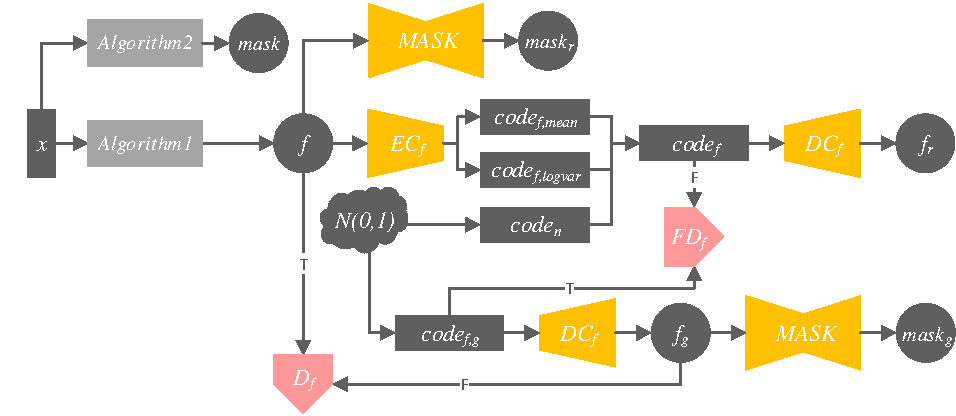
\includegraphics[width=0.95\columnwidth]{figures/feature_train}
	\caption{Structural Feature Map Generation Training.}
	\label{feature_train}
\end{figure}
\begin{algorithm}
	\caption{Mask Extraction}
	\label{alg:2}
	\begin{algorithmic}[1]
		\State Input a real image $x$ and expanded pixel value $p$
		\State $mask = 1.0 - ones \times (x > 0.)$
		\State $new\_size=[x.width() + p, x.length() + p]$
		\State $mask = resize(mask, new\_size)$
		\State $mask = crop\_padding(mask,p)$
	\end{algorithmic}  
\end{algorithm}
When generating the structural feature map, \cite{4shin2018medical} still needs to input the real modal image to get the generated structural feature map, which greatly reduces the diversity of generated data. \cite{41costa2017towards} implements a method based on VAE for generating retinal blood vessel distribution maps from multidimensional normal distribution. Drawing on this, we design a hybrid network combining the characteristics of VAE and GAN for generating brain structural feature maps from random normal distribution matrixes, which has better diversity and no additional training data. In addition,  we train a generator $MASK$ that acquires the brain area masks from the brain structure feature maps for later use to match lesion label. The generator is synchronized with the training of structural feature map generation. During the training of $MASK$, the mask extracted by the real brain MRI $x$ through the mask extraction algorithm (Algorithm~\ref{alg:2}) is used as label data. As shown in Fig.~\ref{feature_train}, the specific training processing is as follows:
\begin{itemize}
	\item The structural feature map $f$ is obtained from $x$ using Algorithm~\ref{alg:1}, and the mask $mask$ is obtained by the Algorithm~\ref{alg:2};
	\item Encode $f$ with VAE encoder $EC_f$ to get $code_{f,mean}$ and $code_{f,logvar}$, then get a random noise $code_n$ from multidimensional normal distribution $\mathcal{N}(0,1^2)$, so the approximate normal distribution matrix  $code_f=code_{f,mean}+exp(0.5\times code_{f,logvar})\times code_n$;
	\item Decode $code_f$ with VAE decoder $DC_f$ to obtain the reconstructed structural feature map $f_r$;
	\item Use mask generator $MASK$ to extract mask $mask_r$ from $f$;
	\item Randomly generate a matrix $code_{f,g}$ that obeys normal distribution $\mathcal{N}(0,1^2)$;
	\item Decode $code_{f,g}$ with VAE decoder $DC_f$ to get the generated random structure feature map $f_g$;
	\item Use mask generator $MASK$ to extract mask $mask_g$ from $f$;
	\item Structural feature discriminator $D_f$ identifies $f$ and $f_g$ respectively, the former is a positive sample and the latter is a negative sample;
	\item Code matrix distribution discriminator $FD_f$ discriminates between $code_{f,g}$ and $code_f$, the former is a positive sample and the latter is a negative sample.
\end{itemize}

Where, for the constraint of approximate normal distribution matrix, we do not use the original VAE encoder loss, but add a code matrix distribution discriminator to provide adversarial loss for VAE encoder.Meanwhile, we use $L2$ regular loss to guide the mean matrix with a mean of 0 and the variance deviation matrix with a mean of 1.
The complete loss items are as follows, where $\omega_{i,j}$ is the weight of each loss item,$mean()$ is the mean function: 
\begin{itemize}
	\item \textbf{Code matrix distribution discriminator loss} 
	\begin{center}
		$loss_{code,d,f}=\Vert{FD_f(code_{f,g})-1}\Vert_{2}^{2}+\Vert{FD_f(code_f)}\Vert_{2}^{2}$
	\end{center}
	
	\item \textbf{Structural feature map discriminator loss} 
	\begin{center}
		$loss_{d,f}=\Vert{D_f(f)-1}\Vert_{2}^{2}+\Vert{D_f(f_g )}\Vert_{2}^{2}$
	\end{center}
	
	\item \textbf{Structural feature map adversarial loss} 
	\begin{center}
		$loss_{g,f}=\Vert{FD_f(code_f)-1}\Vert_{2}^{2}+\Vert{D_f(f_g)-1}\Vert_{2}^{2}$
	\end{center}
	
	\item \textbf{Code matrix distribution loss } 
	\begin{center}
		$loss_{normal}=\Vert{mean(code_{f,mean})}\Vert_{2}^{2}+ \Vert{mean(exp(0.5\times code_{f,logvar}))-1}\Vert_{2}^{2}$
	\end{center}
	
	\item \textbf{Structural feature map reconstruction loss} 
	\begin{center}
		$loss_{reconstruction,f}=\Vert{f-f_r}\Vert_{2}^{2}+\Vert{f_r\times mask}\Vert_{2}^{2}$
	\end{center}
	
	\item \textbf{Mask reconstruction loss}
	\begin{center}
		$loss_{reconstruction,mask}=\Vert{mask-mask_r }\Vert_{2}^{2}+\Vert{f\times mask_r}\Vert_{2}^{2}+\Vert{f_r\times mask_r}\Vert_{2}^{2}+\Vert{f_g\times mask_g}\Vert_{2}^{2}$
	\end{center}
\end{itemize}

\subsection{Reconstruction and translation training}
We perform reconstruction and transformation training on real data and synchronize with the multimodal MRI generation training in subsequent chapters to constrain each component to complete our specified tasks in the multimodal MRI generation process. In addition, we also use a code matrix distribution discriminator $FD$ to guide the consistency of code matrixes distribution between the two training processes. All discriminator components are updated independently, the discriminator training process is shown in Fig.~\ref{train_D}

\begin{figure}
	\centering
	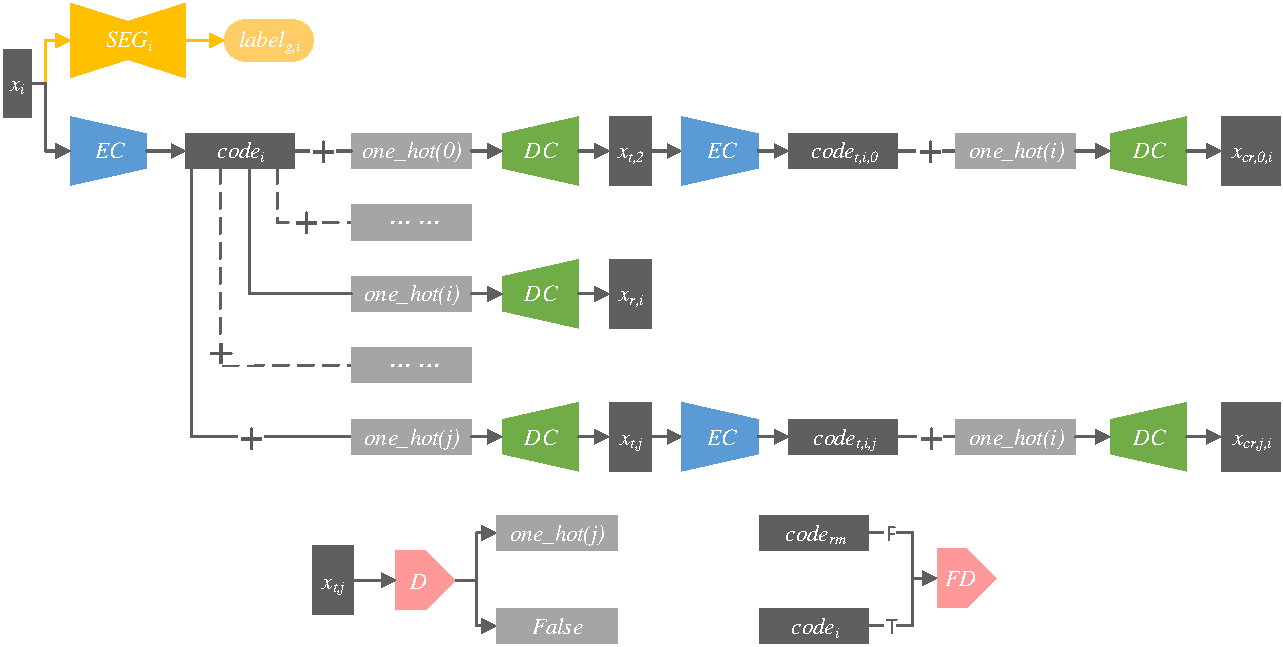
\includegraphics[width=0.95\columnwidth]{figures/trans_train}
	\caption{Reconstruction and translation training.}
	\label{trans_train}
\end{figure}

As shown in Fig.~\ref{trans_train}, when the MRI is reconstructed and translated, the encoder $EC$ encodes the real MRI $x_i$ of modality $i$ to obtain the semantic feature map $code_{i}$, then we connect it to different conditional matrixes and decode all the modalities through the decoder $DC$. In cycle-reconstruction, we use encoder to re-encode all the obtained translation images, connect all the re-encoded semantic feature maps with the conditional vector of modality $i$, and finally decode them by decoder to get cycle-reconstruction image $x_{rc,j,i}$. In the above process, we use the lesion label $l_i$ of the original input modality $x_i$ as supervised label for the lesion generation training, and use lesion label generation components for $x_i$ to get $l_{r,i}$.

The detailed losses are as follows, where $x_{t,j,i}$ refers to MRI $x_i$ of modality $i$ translated by modality $j$; $d_{t, j, i}$ and $c_{t, j, i}$ are the True/False discrimination and category discrimination results of the discriminator $D$ for $x_{t, i, j}$; $code_{t,i,j}$ represents the semantic feature map obtained from $x_{t,i,j}$ by encoder:
\begin{itemize}
	\item \textbf{Discriminator loss}
	\begin{center}
		$loss_{d,1}=\sum\limits_{j=0,j\neq i}\sum\limits_{i=0}(\Vert{d_{t,j,i}}\Vert_{2}^{2}+\Vert{c_{t,j,i}-i}\Vert_{2}^{2})+
		\sum\limits_{i=0}(\Vert{FD(code_{i})-1}\Vert_{2}^{2})$
	\end{center}
	
	\item \textbf{Adversarial and category guidance loss}
	\begin{center}
		$loss_{g,1}=\sum\limits_{j=0,j\neq i}\sum\limits_{i=0}(\Vert{d_{t,j,i}-1}\Vert_{2}^{2}+\Vert{c_{t,j,i}-i}\Vert_{2}^{2})$
	\end{center}
	
	\item \textbf{MRI reconstruction loss}
	\begin{center}
		$loss_{reconstruction}=\sum\limits_{i=0}(\Vert{x_i-x_{r,i}}\Vert_{2}^{2})$
	\end{center}
	
	\item \textbf{MRI cycle-reconstruction loss}
	\begin{center}
		$loss_{cycle}=\sum\limits_{j=0,j\neq i}\sum\limits_{i=0}(\Vert{x_i-x_{cr,j,i}}\Vert_{2}^{2})+\sum\limits_{k=0,k\neq j,k\neq i}\sum\limits_{j=0,j\neq i}\sum\limits_{i=0}(\Vert{x_{cr,j,i}-x_{cr,k,i}}\Vert_{2}^{2})$
	\end{center}
	
	\item \textbf{Semantic consistency loss}
	\begin{center}
		$loss_{code,1}=\sum\limits_{j=0,j\neq i}\sum\limits_{i=0}(\Vert{code_i-code_{t,i,j}}\Vert_{2}^{2})$
	\end{center}
	
	\item \textbf{Lesion segmentation loss}
	\begin{center}
		$loss_{lesion,1}=\sum\limits_{i=0}\Vert{label_i-label_{r,i}}\Vert_{2}^{2}$
	\end{center}
	
\end{itemize}

\subsection{Structural feature map and lesion label fusion}

First we generate structural feature map $f_g$, then randomly select the appropriate lesion segmentation label $label$, and then the lesion segmentation label containing $n$ categories is converted into a one-hot matrix $onehot_l$ of $n$ channels, and each channel corresponds to a segmentation category, the pixel value in each channel is 0 or 1. Each 1 pixel area is registered with each segmentation area in the original segmentation label. At last, we calculate the weighted sum of each channel of $onehot_l$ with $f_g$, and get a new matrix that fuses the information of $f_g$ and $label$.

If the structural feature map $f'$ is extracted from the random MRI $x$, then the extracted structural features may contain tumor structure information, which may interfere with the tumor information at random label $l$ and affect the fusion generation MRI, so $f'$ needs to eliminate the tumor information before fusing with the random label $label$, and get the structural feature map $f$ without tumor information, so that the tumor information of the generated image is only derived from the label $label$. We generate a mask without boundary expansion $mask_{l,x}$ for segmentation label $label_x$ of $x$ by the Algorithm~\ref{alg:2}, then we have $f=mask_{l,x}\times f'$.

Since the location of the randomly selected lesion may appear outside the brain contour of structural feature map, we need to use the Algorithm~\ref{alg:2} to obtain the brain region mask $mask$ of the structural feature map. If the product of $mask$ and the selected $label$ is 0, then the tumor label pixel is inside the brain contour of $mask$, which can be adopted, otherwise the $label$ needs to be re-selected.

\subsection{Multimodal MRI generation training}
\begin{figure}
	\centering
	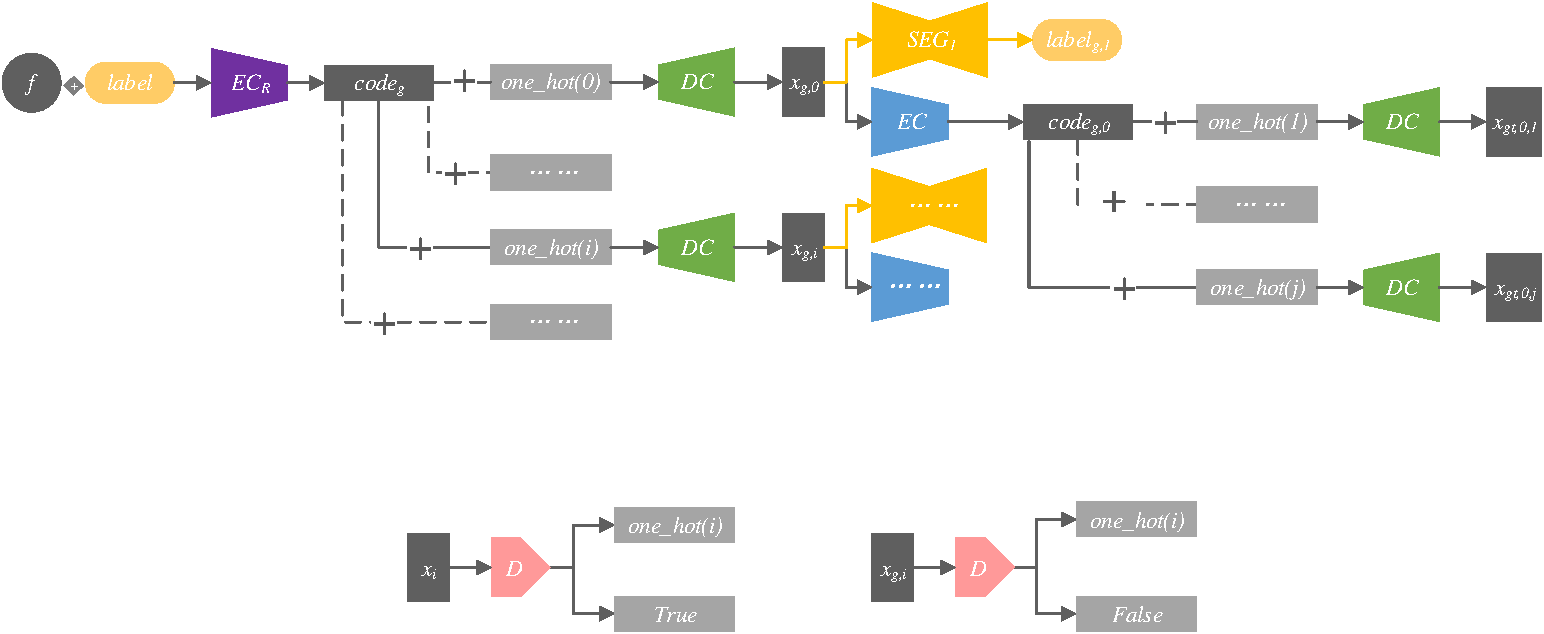
\includegraphics[width=0.98\columnwidth]{figures/mm_mri_generate}
	\caption{Generation of multimodal MRI.}
	\label{mm_mri_generate}
\end{figure}

\begin{figure}
	\centering
	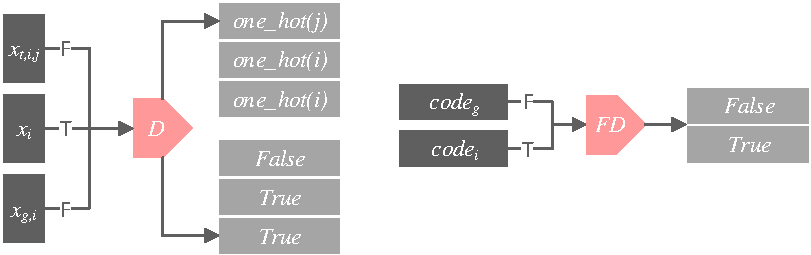
\includegraphics[width=0.75\columnwidth]{figures/D}
	\caption{Discriminator training during reconstruction and translation training on real MRI and multimodal MRI generation training.}
	\label{train_D}
\end{figure}
We extract the structural feature map $f$ from the real MRI by the Algorithm~\ref{alg:1}, and randomly select the real lesion label $label$ to fusion. The fusion map contains basic anatomical information and lesion information of the target site. The multimodal MRI generation process is shown in Fig.~\ref{mm_mri_generate}. First, we use a fusion map encoder $EC_r$ to encode fusion map to obtain the semantic feature map. The semantic feature map is stacked with different one-hot conditional matrixes and decodes by MRI decoder to obtains synthesis images of different modalities. These synthesis images are then perform modal translation process between each other by MRI encoder and MRI decoder. We use adversarial loss and category guidance loss provided by MRI discriminator to constrain synthesis image to approximate real MRI, and constrain the consistency of all semantic feature maps and translation images by loss, thus ensuring the mutual registration of generated multimodal MRI. In addition, we used the lesion label generation components to segment the tumor lesion segmentation labels from each synthetic MRI to ensure that the generated multimodal images have generated corresponding lesion content based on the input lesion label. The lesion label generation components are only trained by real data in synchronous reconstruction and translation training. 

The specific loss items are as follows, where $d_{i}$ and $c_{i}$ are the True/False discrimination and category discrimination of the discriminator $D(x_i)$, $d_{g, i}$,$c_{g,i}$ is the output of $D(x_{g,i})$; $x_{g,i}$ is the synthetic image of modality $i$, $x_{gt,j,i}$ is the translation image of the modality $i$ translated by synthetic image of modality $j$; $code_g$ is the semantic feature map obtained by fusion map encoder$EC_R$, $code_{g,i}$ is the semantic feature map encoded from $x_i$; $l$ is the input label, $l_{g,i}$ is the label obtained by lesion label generation component from $x_{g,i}$; $f$ is the input structural feature map, $f_{g,i}$ is the structural feature map extracted from $x_{g,i}$ by Algorithm~\ref{alg:1}:
\begin{itemize}
	\item \textbf{Discriminator loss }
	\begin{center}
		$loss_{d,2}=\sum\limits_{i=0}(\Vert{d_{i}-1}\Vert_{2}^{2}+\Vert{d_{g,i}}\Vert_{2}^{2}+\Vert{c_{i}-i}\Vert_{2}^{2}+\Vert{c_{g,i}-i}\Vert_{2}^{2})+\Vert{FD(code_{g})}\Vert_{2}^{2}$
	\end{center}

	\item \textbf{Adversarial and category guidance loss}
	\begin{center}
		$loss_{g,2}=\sum\limits_{i=0}(\Vert{d_{g,i}-1}\Vert_{2}^{2}+\Vert{c_{g,i}-i}\Vert_{2}^{2})+\Vert{FD(code_{g})-1}\Vert_{2}^{2}$
	\end{center}
	
	\item \textbf{Structural feature map consistency loss}
	\begin{center}
		$loss_{f}=\sum\limits_{i=0}(\Vert{f-f_{g,i}}\Vert_{2}^{2})$
	\end{center}
	
	\item \textbf{Lesion generation loss}
	\begin{center}
		$loss_{lesion,2}=\sum\limits_{i=0}(\Vert{label-label_{g,i}}\Vert_{2}^{2})$
	\end{center}
	
	\item \textbf{MRI registration loss}
	\begin{center}
		$loss_{registration}=\sum\limits_{j=0,j\neq i}\sum\limits_{i=0}(\Vert{x_{g,i}-x_{gt,j,i}}\Vert_{2}^{2})$
	\end{center}
	
	\item \textbf{Semantic consistency loss}
	\begin{center}
		$loss_{code,2}=\sum\limits_{i=0}(\Vert{code_g-code_{g,i}}\Vert_{2}^{2})+\sum\limits_{j=0,j\neq i}\sum\limits_{i=0}(\Vert{code_{g,i}-code_{g,j}}\Vert_{2}^{2})$
	\end{center}
	
\end{itemize}

\subsection{Lesion generation guidance method}
\label{label gen methods}
As shown in Fig.~\ref{segmentation}, we design the following three lesion label generation components to provide guidance loss for lesion generation in multimodal MRI generation training:
\begin{itemize}
	\item \textbf{Single segmentor} 
	Each MRI modality  is segmented by a common complete segmentor $SEG$.
	\item \textbf{Single lesion encoder + multiple lesion decoders} 
	Each MRI modality  is segmented by a segmentors which is combined by a common lesion encoder $EC_{l}$ and different lesion decoders $EC_{l,i}$. 
	\item \textbf{Multiple segmentors} 
	Each MRI modality  is segmented by a different complete segmentor $SEG_i$.
\end{itemize}
The loss item of the above three schemes in reconstruction and translation training is consistent with the loss item described above. And in the generation training, they only provide the same lesion label generation loss for MRI generation components, no learning.

\begin{figure}
	\centering
	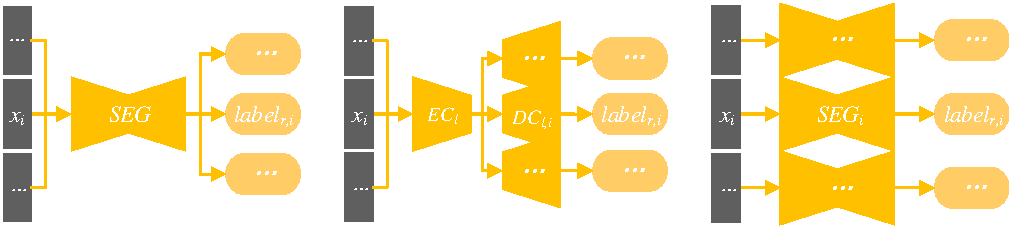
\includegraphics[width=0.8\columnwidth]{figures/segmentation}
	\caption{Lesion segmentation.}
	\label{segmentation}
\end{figure}
Besides, we will also independently train the segmentors of these three schemes. In different experiments, we will train the segmentor in each scheme with different amounts of synthetic data or real data. The loss function of the training is as follows, where $label_i$ is the supervised label and $label_{r,i}$ is the segmentation result:
\begin{center}
	$loss_{segmentation}=\sum\limits_{i=0}\Vert{label_i-label_{r,i}}\Vert_{2}^{2}$
\end{center}

\subsection{Constructing synthetic datasets}
\label{make dataset}
\begin{figure}
	\centering
	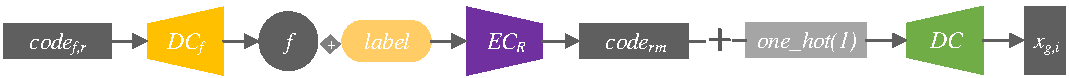
\includegraphics[width=0.98\columnwidth]{figures/make_data}
	\caption{Construction of synthetic datasets.}
	\label{make_data}
\end{figure}
As shown in Fig.~\ref{make_data}, we can generate any number of structural feature maps from randomly generated normal distribution matrix through the trained structural feature map decoder. Then, we randomly scaled, rotated, translated, flipped, etc. the original set of labels to get a random lesion label set. We then fuse the generated structural feature map with the randomly selected label from the random lesion label set. Like training, we can select suitable labels by obtaining mask from structural feature map through the mask generator $MASK$.

Due to the influence of the operation that removing tumor information during training, there are some structural feature maps with poor quality that brain contour is not closed, so we design a structural feature map filtering algorithm for this. First, we use the generator $MASK$ to generate the mask of structural feature map. Then, we perform Gaussian blur\cite{92wink2004denoising} on the structural feature map, and use the contour search algorithm and filling algorithm provided by OpenCV\footnote{https://opencv.org/} to obtain all the closed contours of the Gaussian blur image and fill them. So we get another mask by the traditional algorithm. Finally, we calculate the Mean Absolute Error (MAE) of the two masks. If the MAE is lower than the threshold we set, that means the main brain contour of the structural feature map is relatively complete, and the feature map can be used; otherwise, it means that the mask obtained by the traditional algorithm is hollow inside and quite different with the mask generated by the generator, so it needs to be regenerated. The algorithm is expressed as Algorithm~\ref{alg:3}.
\begin{algorithm}
	\caption{Structural feature map filtering}
	\label{alg:3}
	\begin{algorithmic}[1]
		\State Input a MAE threshold $mae$
		\State \textbf{function} $get\_mask(f)$
		\State \indent$contours = OpenCV.findContours(f)$
		\State \indent$mask =OpenCV.drawContours(f,contours)$
		\State \indent\textbf{return} $mask$
		\State \textbf{do} 
		\State \indent$f = DC_f()$
		\State \indent$m = MASK(f)$
		\State \indent$m'= get\_mask(f)$
		\State \textbf{while} $MAE(m',m) <= mae$
	\end{algorithmic}  
\end{algorithm}

In the generated multimodal MRIs, there still are samples with poor lesion generation. At this point, we segment our synthetic MRI data through the lesion segmentor pre-trained on real data.We filter according to the segmentation evaluation score(default threshold is 0.95 on dice score). After multiple filtering, we obtain the final synthetic dataset consisting of structural feature maps, masks,  lesion segmentation labels, and multimodal MRI.

\section{Experiments}

\subsection{BRATS2015 dataset}
We use the open dataset BRATS2015\cite{91menze:hal-00935640} for experiments, which has four registered modalities of T1/T2/T1c/Flair. The training dataset contains 274 3D MRIs per modality, with the size of 155$\times$240$\times$240, and 274 tumor segmentation labels of the same size. We divide the sample into a training set and a testing set by 9:1, and construct a 2D data set from 50 slices of each 55-105 of the 3D MRI. In data preprocessing, we standardized each image.

\subsection{BRATS synthetic dataset}
We constructed a registered synthetic dataset with tumor labels containing four modalities of T1/T2/T1c/Flair using the method in ~\ref{make dataset}. The size of the synthetic dataset samples is consistent with the BRATS2015 dataset, but the number of samples can be any number according to the needs of the experiment.

\subsection{BRATS enhanced dataset}
We performed random scaling, rotation, translation, flipping, etc. on the original BRATS2015 dataset to obtain enhanced data. The size of the enhanced dataset sample is consistent with the BRATS2015 dataset, but the number of samples can be any number according to the needs of the experiment.

\subsection{Training settings}
The number of iterations of each experiment is equal to 100 epochs of the BRATS2015 training dataset. The learning rate is 1e-4 without weight decay.  we use Adam optimizer with beta1 of 0.5 and perform a Dropout of 0.1 on the input layer, Batch size is 1. We used Dice Score \cite{95dice1945measures} and Mean Square Error (MSE)\cite{94prasad1990the} to evaluate the segmentation results. The evaluation results are the average of the 4 modals results on the 2D images, and each experiment is trained four times to retain the best results.

\subsection{Experiments of lesion generation methods}
\label{label gen methods tests}
As shown in the Table~\ref{label_test}, we trained 4 tumor lesion segmentors using the Multiple segmentors scheme on the BRATS2015 training dataset and test them on the BRATS2015 testing dataset. Then we used the trained segmentors to segment the unfiltered synthetic data from different lesion generation guidelines.

\subsection{Experiments of synthetic data availability}
As shown in the Table~\ref{availability_test}, we mixed real BRATS2015 training data with BRATS synthetic data in different amounts, then used the mixed dataset for segmentation training using the Multiple segmentors scheme, and evaluated the segmentation ability of the model on real BRATS2015 testing dataset. All experiments were fully trained with the same number of iterations, which equal the number of 100 epochs on BRATS2015 training dataset. At the same time, we set up three data mixing modes: random mixing, real data training first, and synthetic data training first. And in real first experiments and synthetic first experiments, the training iteration steps of data from different sources is proportional to the amount of data. Except the conditions in tabel, other conditions are identical.

\section{Results}
\subsection{Results of Lesion generation methods}
\begin{table}[t]
	\caption{Lesion generation methods experiments}\smallskip
	\centering
	\resizebox{.75\columnwidth}{!}{		
		\smallskip\begin{tabular}{llll}		
			\toprule	
			segmentation schemes&testing dataset &MSE   &Dice Score \\	
			\midrule		
			4 $SEG$&real 		   				&0.026 &0.915 \\					
			1 $SEG$&synthetic     			&0.053 &0.741 \\			
			1 $EC_{lesion}$ + 4 $DC_{lesion}$&synthetic     	&0.055 &0.808 \\		
			4 $SEG$&synthetic     			&0.043 &0.838 \\
			\bottomrule			
		\end{tabular}	
	}	
	\label{label_test}	
\end{table}

As shown in the Table~\ref{label_test}, the segmentation test results reach the MSE 0.026 and the Dice Score 0.915 of the segmentors trained on the real data. From results, three different lesion label generation methods have achieved good segmentation results, where the Multiple segmentors scheme is best. 

\subsection{Results of synthetic data availability}
\begin{table}[t]
	\caption{Synthetic data availability verification experiments}\smallskip
	\centering
	\resizebox{.95\columnwidth}{!}{
		\smallskip\begin{tabular}{lllllll}
			\toprule
			NO. &real data &synthetic data & enhanced data  & mixing modes  & MSE &Dice Score\\
			\midrule
			1 & $\times$1  	 	& 0 		&0 			&- &0.026 &0.915 \\
			2 & $\times$50\% 	 & 0  		&0 			&- &0.032 &0.902 \\
			3 &0 	 	 & $\times$1  	&0 			&- &0.205 &0.708 \\
			4 &0 	 	 & $\times$2  	&0 			&random mixing &0.206 &0.736 \\
			5 &0 		 & $\times$3  	&0 			&random mixing &0.205 &0.754 \\
			6 & $\times$10\% 	 & $\times$1  	&0 			&synthetic first &0.031 &0.908 \\
			7 & $\times$10\% 	 & $\times$2   &0 			&synthetic first &0.028 &0.907 \\
			8 & $\times$10\% 	 & $\times$3   &0 			&synthetic first &0.030 &0.907 \\	
			9 & $\times$20\% 	 & $\times$80\% 	&0  		&random mixing &0.041 &0.850 \\
			10& $\times$50\% 	 & $\times$50\% 	&0  		&random mixing &0.031 &0.904 \\
			11& $\times$80\% 	 & $\times$20\% 	&0  		&random mixing &0.024 &0.935 \\
			12& $\times$1 	 	& $\times$20\% &0  		&random mixing &0.025 &0.921 \\
			13& $\times$1 	 	& $\times$50\% &0  		&random mixing &0.023 &0.939 \\
			14& $\times$1 	 	& $\times$80\% &0  		&random mixing &0.026 &0.916 \\
			15& $\times$1 	 	& $\times$1    &0   		&random mixing &0.027 &0.913 \\
			16& $\times$1 	 	& $\times$2   &0 			&random mixing &0.033 &0.901 \\
			17& $\times$1 	 	& $\times$3   &0 			&random mixing &0.034 &0.897 \\	
			18& $\times$1 	 	&0 		&  $\times$20\%	 	&random mixing &0.027 &0.911 \\
			19& $\times$1 	 	&0 		&  $\times$50\% 	&random mixing &0.025 &0.927 \\
			20& $\times$1    	&0 		&  $\times$80\% 	&random mixing &0.026 &0.920 \\
			21& $\times$1 	 	&0 		&  $\times$1    &random mixing &0.026 &0.915 \\
			22& $\times$1 	 	&0 		&  $\times$2   &random mixing &0.032 &0.898 \\
			23& $\times$1 	 	&0 		&  $\times$3   &random mixing &0.036 &0.885 \\			
			24& $\times$1 	 	& $\times$1 	&0  		&real first &0.195 &0.795 \\
			25& $\times$1 	 	& $\times$1 	&0  		&synthetic first &0.021 &0.940 \\
			\bottomrule
		\end{tabular}
	}
	\label{availability_test}
\end{table}
%\begin{table}[t]
%	\caption{Synthetic data availability verification experiments}\smallskip
%	\centering
%	\resizebox{.95\columnwidth}{!}{
%		\smallskip\begin{tabular}{lllllll}
%			\toprule
%			NO. &real data &synthetic data & enhanced data  & mixing modes  & MSE &Dice Score\\
%			\midrule
%			1 & 1Fold  	 & 0  		&0 			&- &0.026 &0.915 \\
%			2 & 50\% & 0  		&0 			&- &0.032 &0.902 \\
%			3 & 0 	 	 & 1Fold  	&0 			&- &0.205 &0.708 \\
%			4 & 0 	 	 & 2Folds  	&0 			&random mixing &0.206 &0.736 \\
%			5 & 0 		 & 3Folds  	&0 			&random mixing &0.205 &0.754 \\
%			6 & 10\% 	 & 1Fold  	&0 			&synthetic first &0.031 &0.908 \\
%			7 & 10\% 	 & 2Folds   &0 			&synthetic first &0.028 &0.907 \\
%			8 & 10\% 	 & 3Folds   &0 			&synthetic first &0.030 &0.907 \\	
%			9 & 20\% 	 & 80\% 	&0  		&random mixing &0.041 &0.850 \\
%			10& 50\% 	 & 50\% 	&0  		&random mixing &0.031 &0.904 \\
%			11& 80\% 	 & 20\% 	&0  		&random mixing &0.024 &0.935 \\
%			12& 1Fold 	 & 0.2Folds &0  		&random mixing &0.025 &0.921 \\
%			13& 1Fold 	 & 0.5Folds &0  		&random mixing &0.023 &0.939 \\
%			14& 1Fold 	 & 0.8Folds &0  		&random mixing &0.026 &0.916 \\
%			15& 1Fold 	 & 1Fold    &0   		&random mixing &0.027 &0.913 \\
%			16& 1Fold 	 & 2Folds   &0 			&random mixing &0.033 &0.901 \\
%			17& 1Fold 	 & 3Folds   &0 			&random mixing &0.034 &0.897 \\	
%			18& 1Fold 	 &0 		&  20\%	 	&random mixing &0.027 &0.911 \\
%			19& 1Fold 	 &0 		&  50\% 	&random mixing &0.025 &0.927 \\
%			20& 1Fold    &0 		&  80\% 	&random mixing &0.026 &0.920 \\
%			21& 1Fold 	 &0 		&  1Fold    &random mixing &0.026 &0.915 \\
%			22& 1Fold 	 &0 		&  2Folds   &random mixing &0.032 &0.898 \\
%			23& 1Fold 	 &0 		&  3Folds   &random mixing &0.036 &0.885 \\			
%			24& 1Fold 	 & 1Fold 	&0  		&real first &0.195 &0.795 \\
%			25& 1Fold 	 & 1Fold 	&0  		&synthetic first &0.021 &0.940 \\
%			\bottomrule
%		\end{tabular}
%	}
%	\label{availability_test}
%\end{table}

As shown in Table~\ref{availability_test}, the results of NO.3-NO.5 show that the synthetic data can not completely replace the real data in training.            
The results of NO.6-NO.8 show that the results of pre-training with a large amount of synthetic data and fine-tuning on a small amount of real data are very close to those of training with complete real data.   
In the experiment NO.9-NO.11, the results of different mixing ratios are also quite different. When the ratio of the two is similar, the segmentation results are similar to experiment NO.1. When the proportion of synthetic data is high, the synthetic data will interfere with the learning of real data, and the result is lower than that of experiment NO.1. When the proportion of synthetic data is low, the generalization ability of the model can be improved by synthetic data, and the result is higher than experiment NO.1.            
In the experiment NO.12-NO.17, we further tried to add synthetic data of different data quantities to the real data. We found that adding a small amount of synthetic data can enhance the learning, and the more synthetic data, the better the enhancement effect, but when the synthetic data reaches a certain percentage and then continue to increase, it will achieve the opposite effect.  
In the experiment NO.18-NO.23, we use the enhanced data generated by the usual data enhancement methods to compare the enhancements of the synthesized data. We found that the two are consistent in the trend of increasing the amount of data and the enhancement effect, but there are some differences in  the change curve between  enhancement effect and the increase in data amount. Overall, the enhanced data is more robust in terms of the sensitivity of the model to the amount of enhanced data, but the upper limit of the enhanced effect of synthetic data is much higher than that enhanced data.   
In experiment NO.24-NO.25, we compared experiment NO.15 and found that the performance of the synthesized data is the best when it is used as pre-training data, and the performance is poor when it is used as supplementary training data set. when using as enhanced data to mixed with real data, the synthesized data can also achieve certain enhancements.

Generally, when there is a large amount of real data, a small amount of synthetic data can be used as enhanced data mixing, or a large amount of synthetic data can be used for pre-training and then training on real data. And when there is less real data, a large number of synthetic data can be used for pre-training, then fine-tuned on a small amount of real data, whose results can compete with the results on complete real data, and this conclusion is consistent with \cite{4shin2018medical}. We do not recommend using synthetic data completely for training, and also do not recommend using synthetic data for supplementary training.

\subsection{Synthetic images}
As Figure~\ref{generated_f} shows the examples of the structural feature map we generated from the random normal distribution matrix. Figure~\ref{generated_mri} shows the examples of generated structural feature maps, generated masks, selected lesion segmentation labels, and generated multimodal MRI.
\begin{figure}
	\centering
	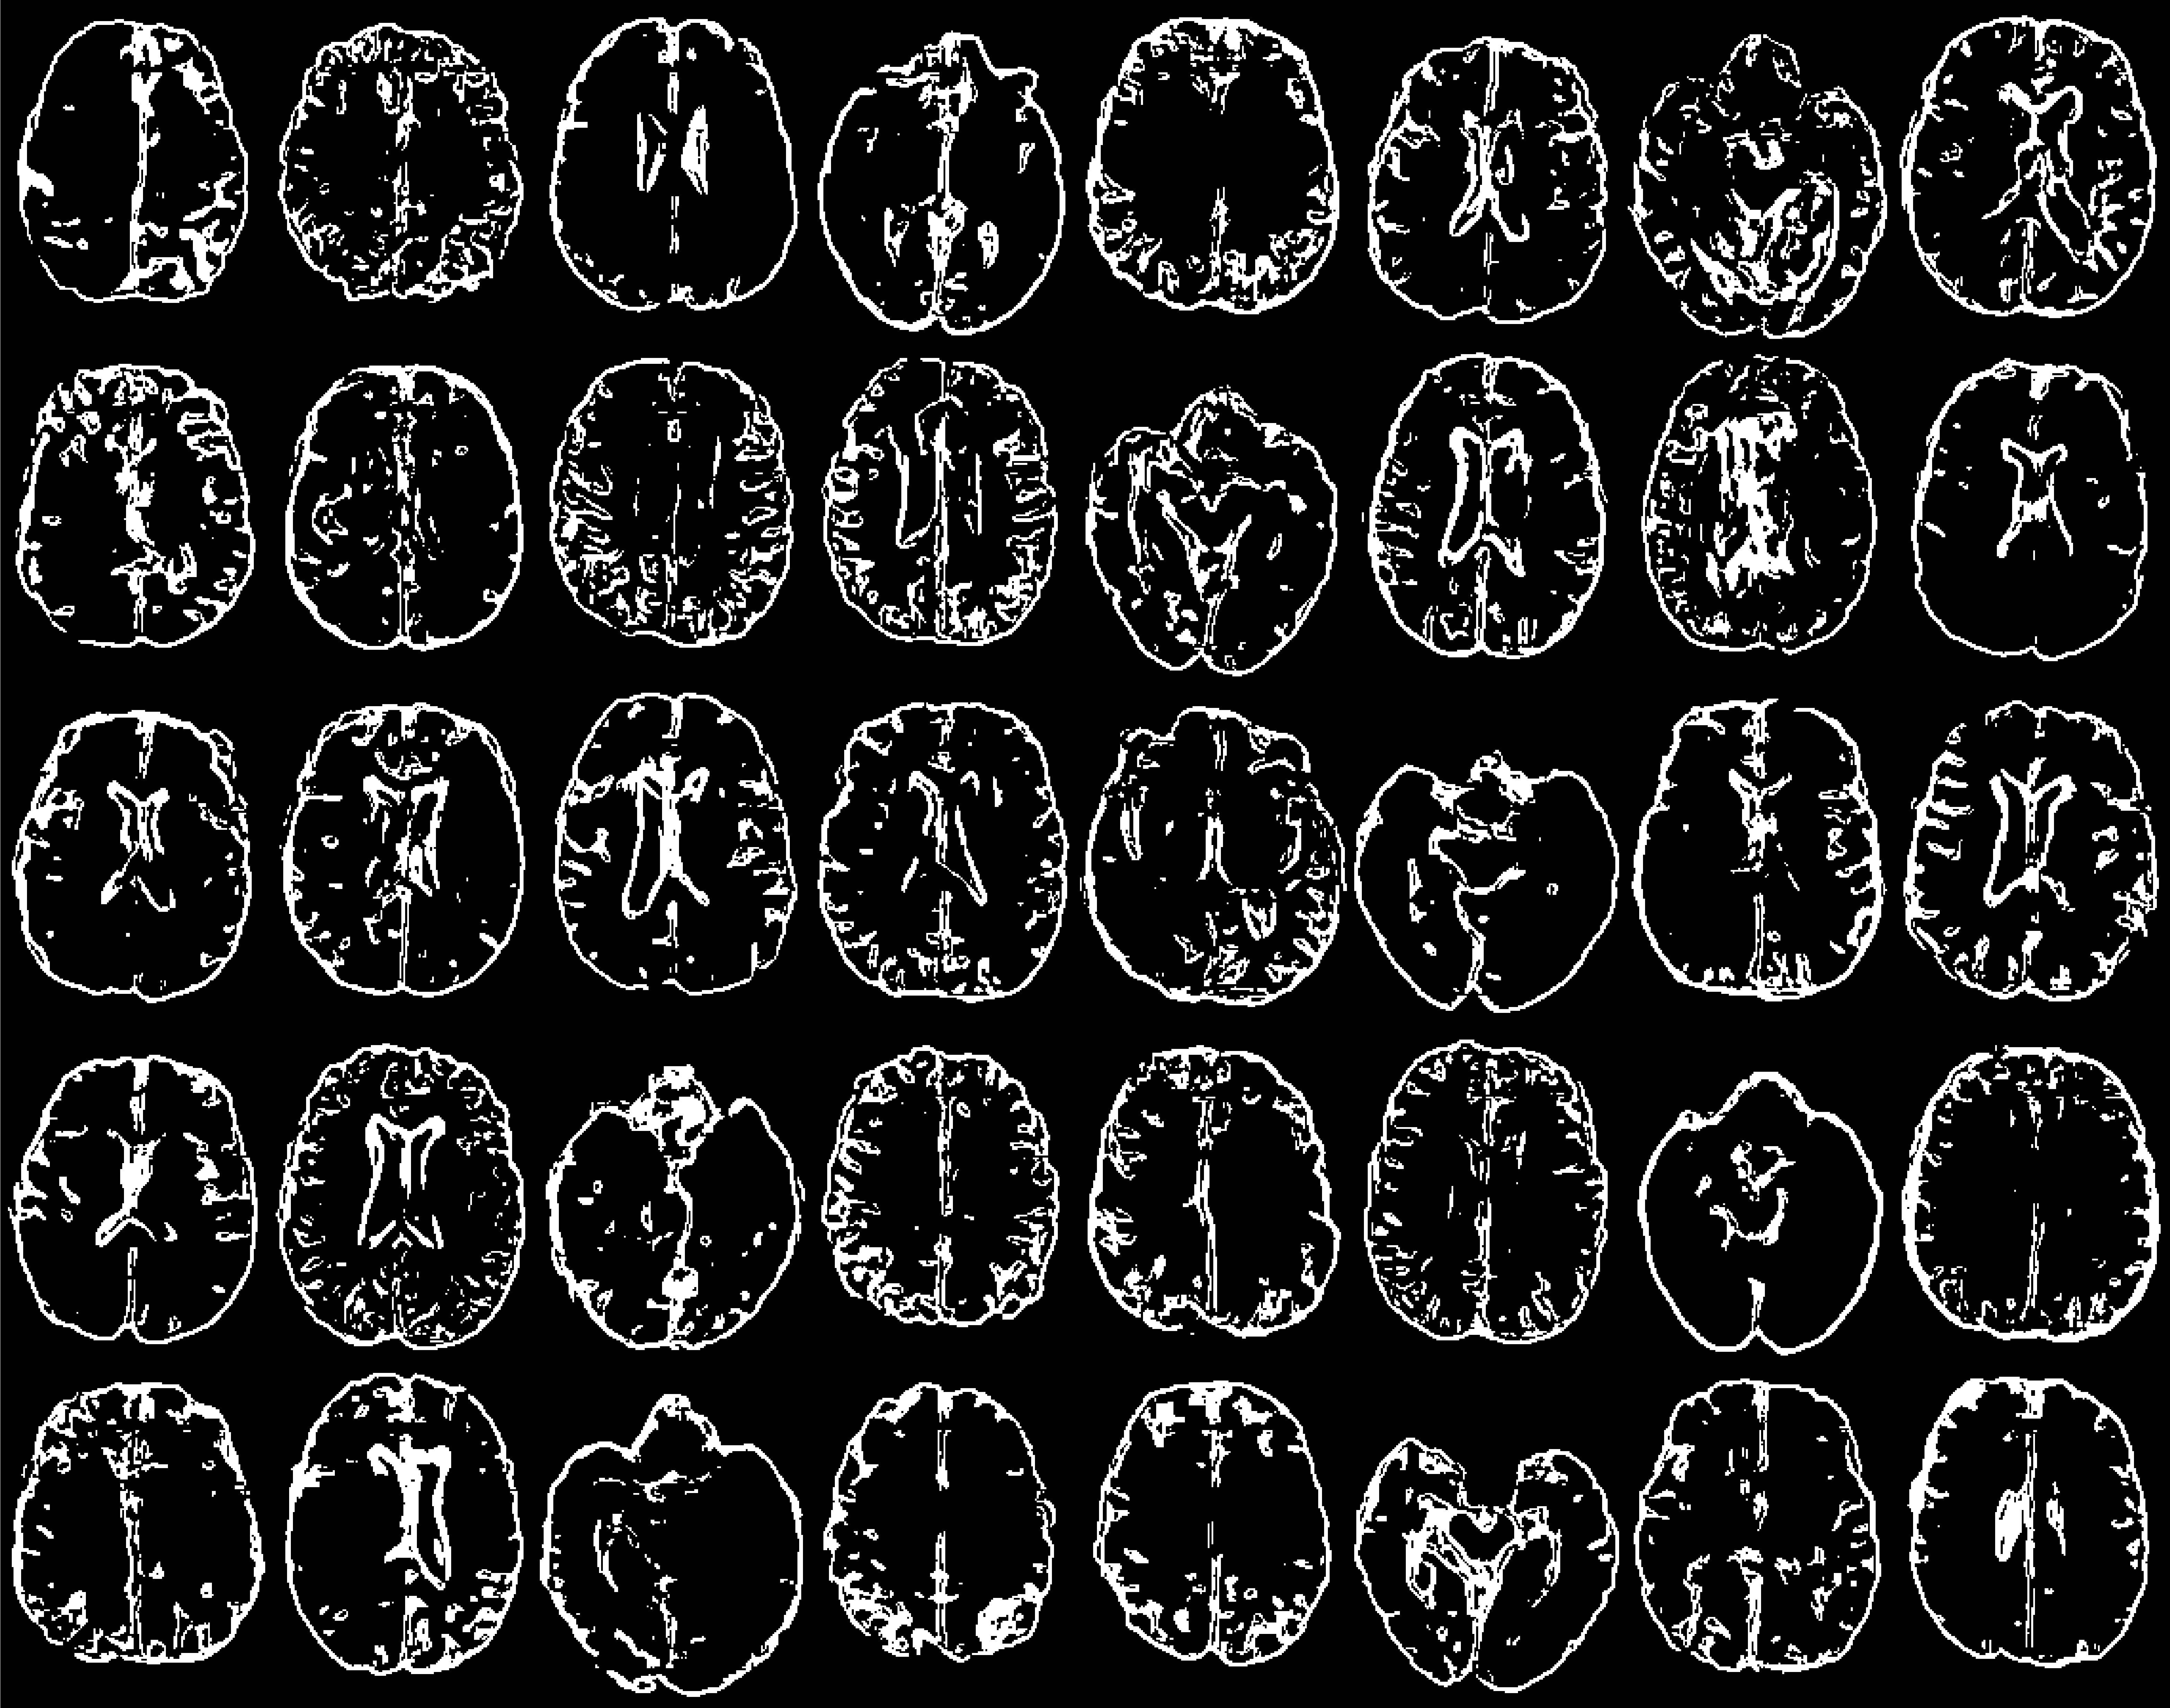
\includegraphics[width=0.7\linewidth]{figures/Fs}
	\caption{Synthetic structural feature maps.}
	\label{generated_f}
\end{figure}

\begin{figure}
	\centering
	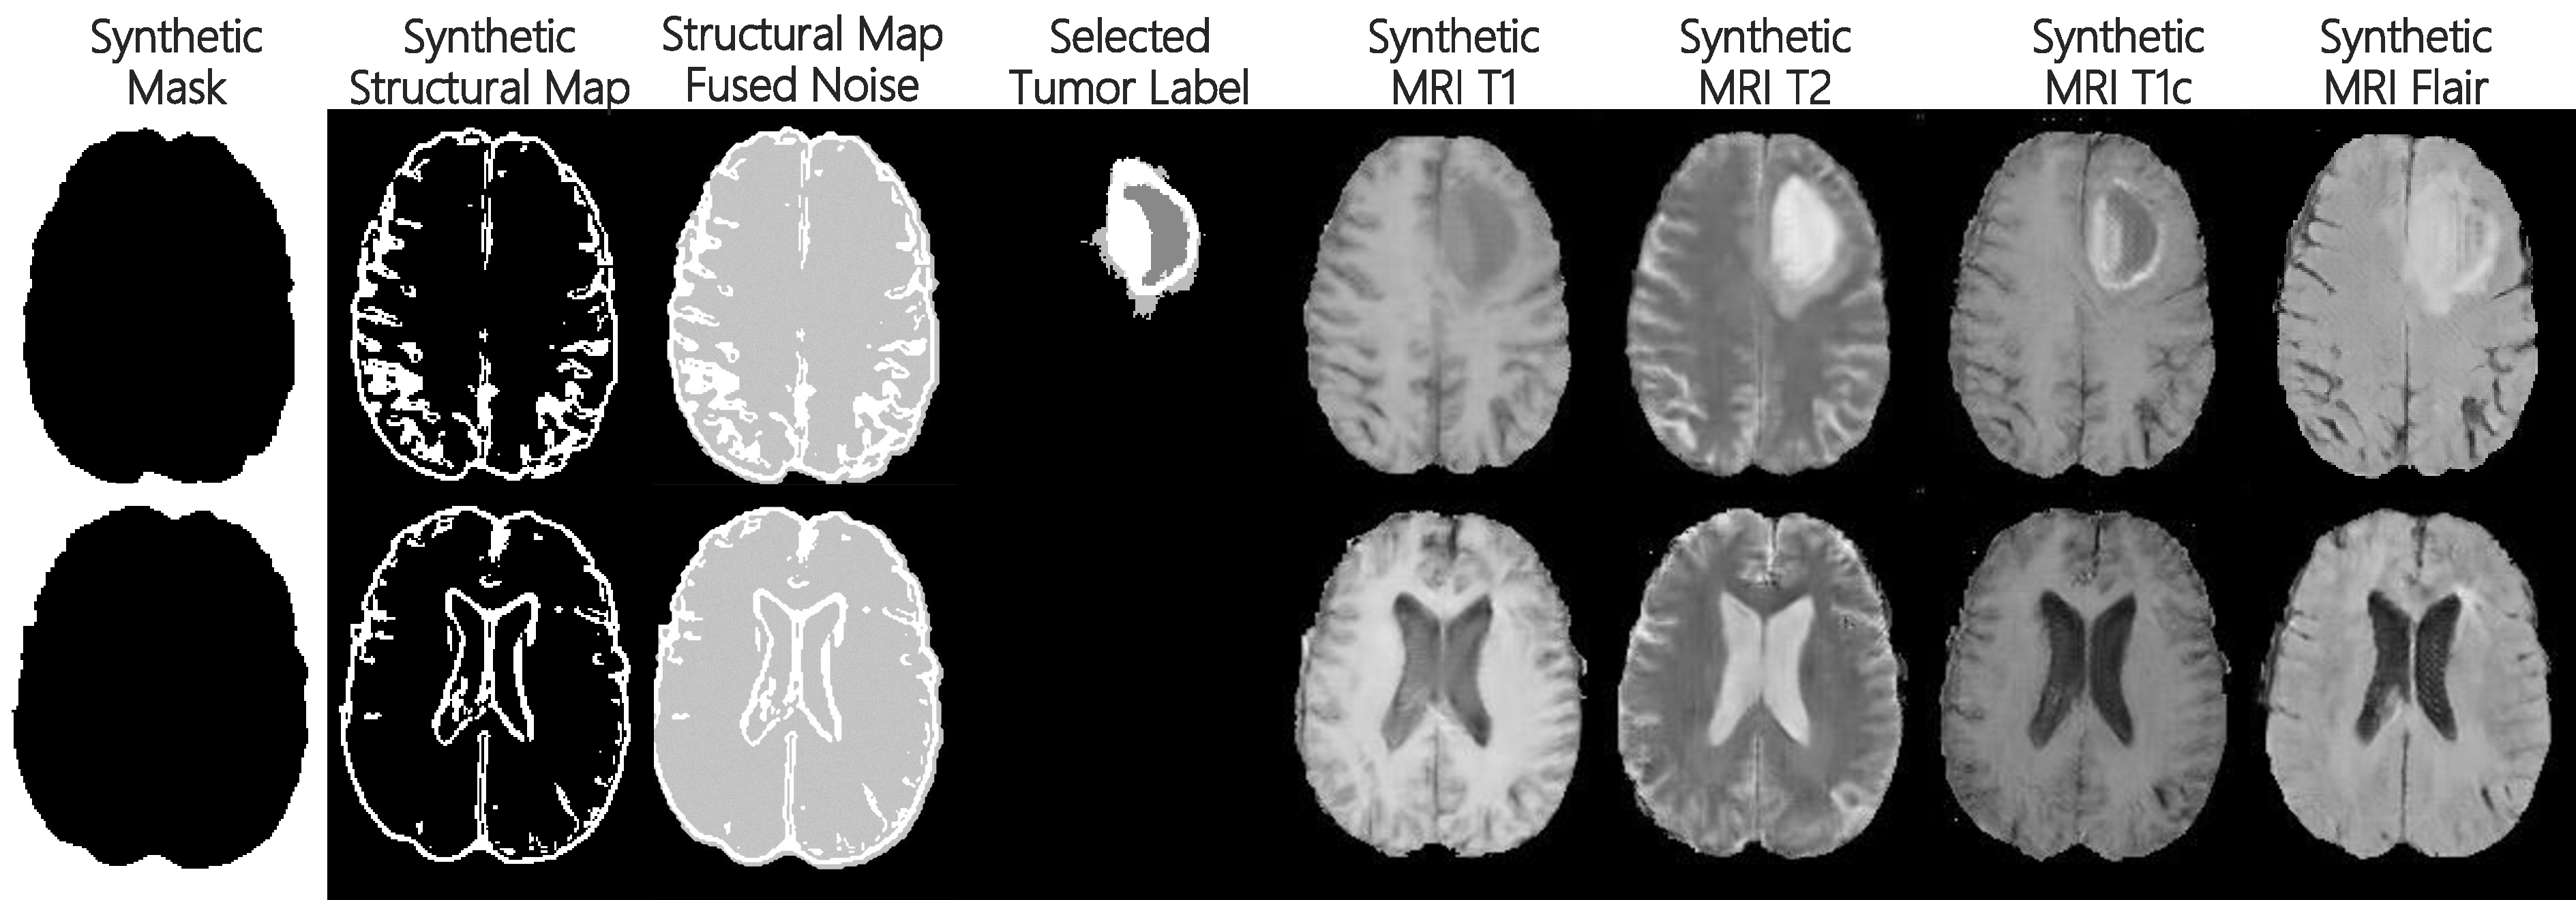
\includegraphics[width=0.8\linewidth]{figures/F_to_MRI}
	\caption{Multimodal MRIs generated from the structural feature maps and lesion labels.}
	\label{generated_mri}
\end{figure}

\section{Conclusion}
Based on the conditional generation antagonism network, we realized the generation of registered multimodal MRI from the random normal distribution matrix through unsupervised training, and could add the lesion information freely. 
We verified through lesion segmentation experiments that synthetic MRI can be used as pre-training data or enhanced data for intelligent medical image processing tasks and can significantly improve the generalization ability of the model.
In this paper, our contributions include the following:
\begin{itemize}
	\item We propose a structural feature map extraction method to extract anatomical structure information directly from medical images without training or additional label data;
	\item We propose a random structure feature map generation method to generate structural feature maps from multi-dimensional normal distribution sampling;
	\item We realized the generation of registered multimodal MRI with corresponding lesion information from structural feature map and randomly selected lesion labels;
	\item We verified that synthetic data can be used as pre-training data or enhanced data for intelligent medical image processing tasks through a number of data usability tests on our synthetic dataset.
	
\end{itemize}

%In the future, we will further improve our method in CT, PET and other modes, in heart, lung and other parts, in detection, classification and other lesion processing tasks. We are committed to further simplifying the training process and synthesizing higher quality medical images.	

%\section{ Acknowledgments}

%Thanks for the computing support provided by NSCCGZ.


\bibliography{refer}
\bibliographystyle{aaai}

\end{document}
